%% laad alle packages en style-opties in:
\documentclass[11pt,a4paper,titlepage]{article}
\usepackage[utf8]{inputenc}
\usepackage[margin=2cm,headheight=13.6cm]{geometry}
\usepackage{color}
\usepackage{listings}
\usepackage{graphicx}
\usepackage{todonotes}
\usepackage{caption}
\usepackage{float}
\usepackage{titling}
\usepackage{pgfkeys}
\usepackage{wrapfig}
\usepackage{booktabs}
\usepackage{adjustbox}
\usepackage{pdflscape}
\usepackage{tabulary}
\usepackage{courier}
\usepackage{graphicx}
\usepackage{subcaption}
\usepackage{multirow}
\usepackage{enumitem}
\usepackage[ampersand]{easylist}
\usepackage{pdfpages}
\usepackage{amssymb}
\ListProperties(Hide=100, Hang=true, Progressive=3ex, Style*=-- ,
Style2*=$\bullet$ ,Style3*=$\circ$ ,Style4*=\tiny$\blacksquare$ )
% ...
%\uspackage{rotating}
\definecolor{mygreen}{RGB}{0,127,0}
\definecolor{mygray}{RGB}{100,100,100}
\definecolor{mymauve}{RGB}{100,32,255}
\definecolor{lgray}{RGB}{230,230,230}
\lstset{ %
  frame=none,
  backgroundcolor=\color{white},   % choose the background color; you must add \usepackage{color} or \usepackage{xcolor}
  basicstyle=\footnotesize\ttfamily,        % the size of the fonts that are used for the code
  breakatwhitespace=false,         % sets if automatic breaks should only happen at whitespace
  breaklines=true,                 % sets automatic line breaking
  captionpos=t,                    % sets the caption-position to bottom
  commentstyle=\color{mygreen},    % comment style
  deletekeywords={...},            % if you want to delete keywords from the given language
  escapeinside={\%*}{*)},          % if you want to add LaTeX within your code
  extendedchars=true,              % lets you use non-ASCII characters; for 8-bits encodings only, does not work with UTF-8
%  frame=single,                    % adds a frame around the code
  keepspaces=true,                 % keeps spaces in text, useful for keeping indentation of code (possibly needs columns=flexible)
  keywordstyle=\color{blue},       % keyword style
  language=,                 % the language of the code
  morekeywords={*,...},            % if you want to add more keywords to the set
  numbers=left,                    % where to put the line-numbers; possible values are (none, left, right)
  numbersep=5pt,                   % how far the line-numbers are from the code
  numberstyle=\tiny\color{mygray}, % the style that is used for the line-numbers
  rulecolor=\color{black},         % if not set, the frame-color may be changed on line-breaks within not-black text (e.g. comments (green here))
  showspaces=false,                % show spaces everywhere adding particular underscores; it overrides 'showstringspaces'
  showstringspaces=false,          % underline spaces within strings only
  showtabs=false,                  % show tabs within strings adding particular underscores
  stepnumber=1,                    % the step between two line-numbers. If it's 1, each line will be numbered
  stringstyle=\color{mymauve},     % string literal style
  tabsize=4,                       % sets default tabsize to 2 spaces
  aboveskip=3mm,
  belowskip=3mm,
}

\usepackage{fancyhdr}
\pagestyle{fancy}
\rhead{Delft University of Technology}
\usepackage{datetime}
\usepackage{moresize}

\newdateformat{monthyeardate}{%
  \monthname[\THEMONTH] \THEYEAR}

\newcommand{\rulebreak}{%
	\par%
	\vspace{0.9cm}%
    \noindent\rule{4cm}{0.4pt}%
    \vspace{1.2cm}%
    \par%
}

\newcommand{\coverpage}[1]{%
	\pagenumbering{roman}%
	\thispagestyle{empty}%
	\lhead{\textsc{Pattern Recognition - Team 27}}%
    \title{Pattern Recognition, Delft University of Technology}%
    \author{Jurriaan Govers BSc, 4163753 \\ Sebastiaan Joosten BSc, 4103513 \\ Stijn van der Smagt BSc, 4306686 }%
    \newgeometry{left=5cm,bottom=2cm,right=5cm,top=2cm}%
	\begin{center}\hspace{0pt}\vfill%
    \uppercase{Pattern Recognition\\
    Delft University of Technology}
	\rulebreak%
    {\Large\textbf{Final Assignment}}
    
    \vspace{0.5cm}
    {\HUGE\textbf{\textit{#1}}}
    
    \vspace{0.5cm}
	\theauthor%
	\par%
	\vspace{0.9cm}%
    \noindent\rule{4cm}{0.4pt}%
    \vspace{0.45cm}
    %\pagebreak
    %\tableofcontents%
	\rulebreak%
    \monthyeardate\today\par
    \hspace{0pt}
	\end{center}%
    \vfill
    \hspace{0pt}
	\pagebreak%
    \restoregeometry%
    \pagenumbering{arabic}%
}



% Custom arguments for /fig command
\pgfkeys{
 /fig/.is family, /fig,
 default/.style = 
  {scale = 1,
   angle = 0},
 scale/.estore in = \figScale,
 angle/.estore in = \figAngle
}
\newcommand{\fig}[2][]{%
	\pgfkeys{/fig, default, #1}%
	\begin{figure}[H]%
    \centering
    \includegraphics[angle=\figAngle,width=\figScale\textwidth]{#2}%
	\end{figure}%
}

\newcommand{\filename}[1]{%
	\texttt{#1}%
}

\newcommand{\vhdl}[1]{%
  \lstinputlisting[language=vhdl]{#1}
}

\newcommand*\paths[1]{\lstset{inputpath=#1}\graphicspath{#1}}



%% code for bibliography
\usepackage{biblatex}
\usepackage{hyperref}
\usepackage{setspace}
\addbibresource{bibr.bib}
\defbibheading{bibempty}{}
\hypersetup{hidelinks,colorlinks=false,breaklinks=true,urlcolor=ocre,bookmarksopen=false,pdftitle={Title},pdfauthor={Author}}
\renewbibmacro*{doi+eprint+url}{%
  \printfield{isbn}%
  \newunit\newblock
  \iftoggle{bbx:doi}
    {\printfield{doi}%
     \iffieldundef{doi}{}{\renewcommand*{\finentrypunct}{\relax}}}
    {}%
  \newunit\newblock
  \iftoggle{bbx:eprint}
    {\usebibmacro{eprint}%
     \iffieldundef{eprint}{}{\renewcommand*{\finentrypunct}{\relax}}}
    {}%
  \newunit\newblock
  \iftoggle{bbx:url}
    {\usebibmacro{url+urldate}%
     \iffieldundef{url}{}{\renewcommand*{\finentrypunct}{\relax}}}
    {}}
%% end code for bibliography

% Magic spellcheck setting comment:
% !TeX spellcheck = en_US

\begin{document}
  \coverpage{Classification of Hand-Written Digits}
  \pagebreak
  
% \section*{Executive Summary}
% Samenvatting over report (weet niet of het er in moet?)

\newpage
\tableofcontents

\newpage
 \section{Introduction}
  \label{Intro}
  This report describes the design and performance of a Pattern Recognition algorithm that is able to classify images of hand-written digits on bank cheques. It considers two cases:
  \begin{itemize}
  	\item \textbf{Case 1: The system is trained only one time, and then used in the field.} This means a large amount of training data is available.
  	\item \textbf{Case 2: The system is trained for each batch of cheques.} This means only a small amount of training data is available.
  \end{itemize}
Although Case 2 provides significantly less data than Case 1 (and this definitely has to be taken into account during the design of the classification system) it is worthy to note that both cases call for a supervised learning approach. \\
The available data will be extracted from the NIST-list, a large dataset containing labelled hand-written digits from 0 to 9. These images will be processed in order to make it easier to handle them. The loading of the list and processing of the images it contains is done in a separate function, named \texttt{myrep.m}. This function is described in detail in section \ref{sec:ImPros}. Implementing the pre-processing in this way enables the inclusion of the image-processing part of the algorithm in a later benchmark test. It also enables the user to keep the pre-processing consistent across the two different cases if desired.\\
\noindent After the processing, two classifiers will be trained, one for each of the aforementioned cases. These classifiers will be stored as $w$, so that they too can be implemented in the benchmark test. The design of these classifiers is described in detail in section \ref{sec:ClasDes}. \\
Both classifiers will be evaluated using various error estimations. This way, some indication of their performance can be made before sending them to the client. \\
\noindent Finally, to simulate the evaluation by the client for both cases, the benchmark test will be conducted by calling \texttt{e = nist\_eval(myrep,w,n)}. The error $e$ this function returns should be less than 5\% for case 1 and less than 25\% for case 2. An overview of the handling of the data as described in this section can be seen in figure \ref{fig:process_flow}.
\begin{figure}[H]
	\centering
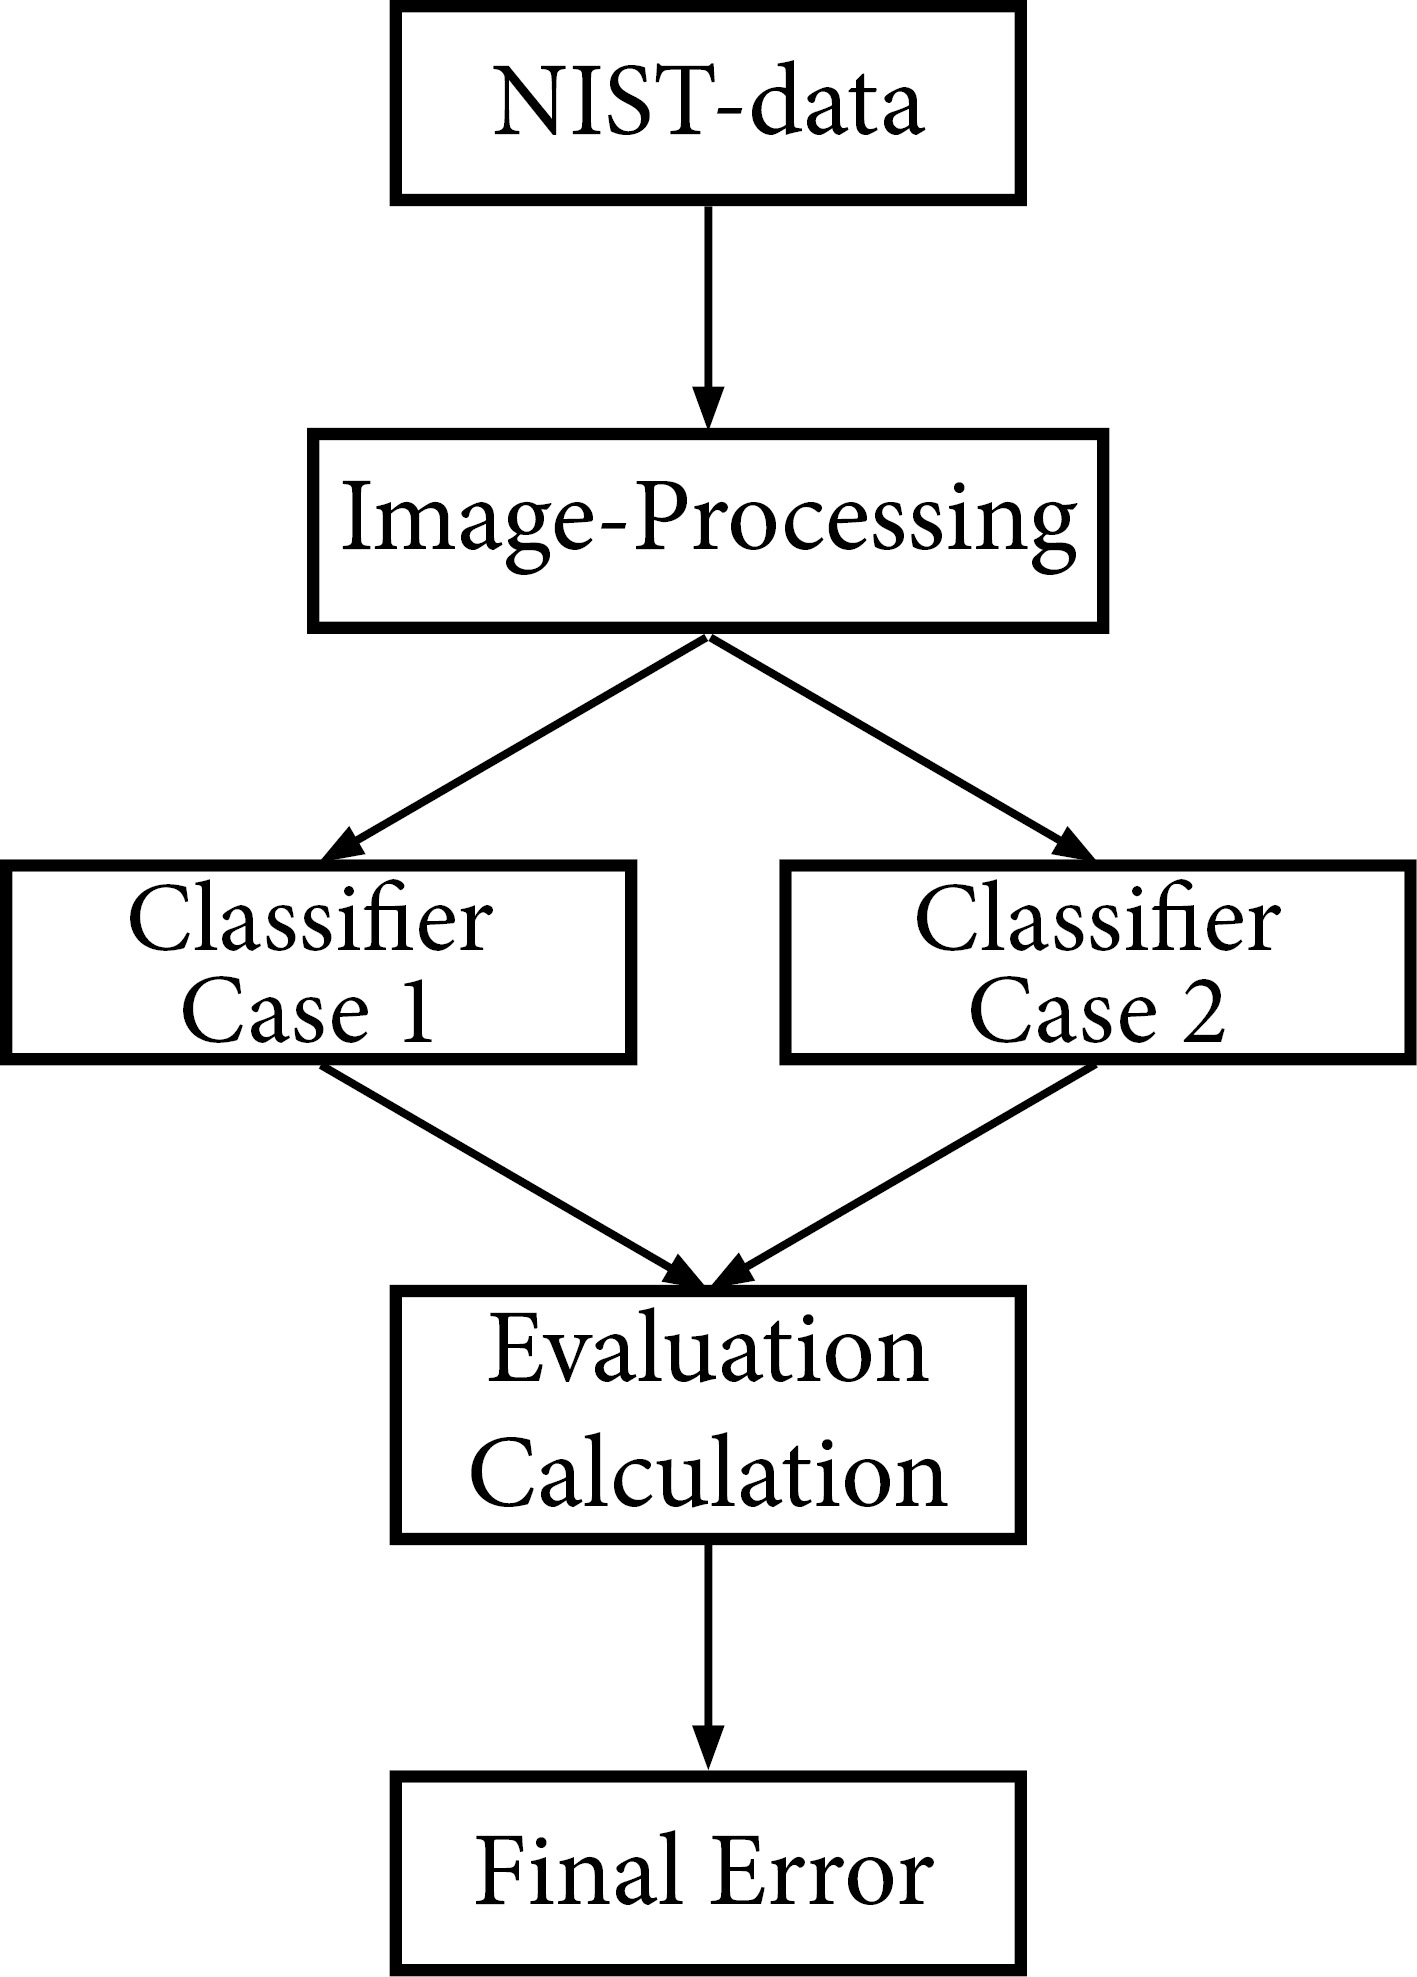
\includegraphics[scale=0.65]{images/Process_Flow.jpg}
\caption{Process of classification of the NIST-data for the two cases.}
\label{fig:process_flow}
\end{figure}
\newpage
\section{Pre-Processing}
\label{sec:ImPros}
Before the classifiers will be trained, some pre-processing is needed. In order to make all images the same size, they were placed within the same bounding box. Next, all images were downsampled to a size of 16 by 16 pixels, to reduce the amount of pixels and save computational time and space. \\
Then some image processing was implemented. When looking at some random samples of the dataset, it was noticed that some of them contained fragmented digits. Also, some spots and blobs could be observed in some images. When using certain Pattern Recognition tools, this could create various problems. For instance, when using a feature-representation to classify the objects, the feature 'perimeter' will look for the first object in every image, and calculate its perimeter. If a small blob is present in the top left corner of an image, it will calculate the perimeter of this blob, and ignore the actual digit. \\
In order to overcome this problem relatively easy, two image processing steps are implemented in the pre-processing phase. First, all images were extracted from the dataset and converted to an image using the \texttt{data2im.m} in MatLab. This means that all kinds of image-processing techniques become available. Since this course focusses on Pattern Recognition, and not so much on Image Processing, it was decided to keep it relatively simple, and just implement two functions to remove some of the spots and blobs. \texttt{bwmorph.m} was used to remove single pixels, and \texttt{bwareaopen.m} was used to remove some larger blobs. After this, the images were converted back to data using \texttt{im2obj.m}, and stored in a prdataset. \\
Finally, a small gaussian filter was used to overcome some 'broken' digits and smooth out some rough edges that originated from the downsampling. While more advanced techniques like image propagation would be more suitable to close for instance sixes and eights, it was decided not to implement this in the interest of time and with the goal of the course in mind. A few examples the pre-processing has on some digits can be seen in figure \ref{fig:Image_Prepros}.
\begin{figure}[H]
	\centering
	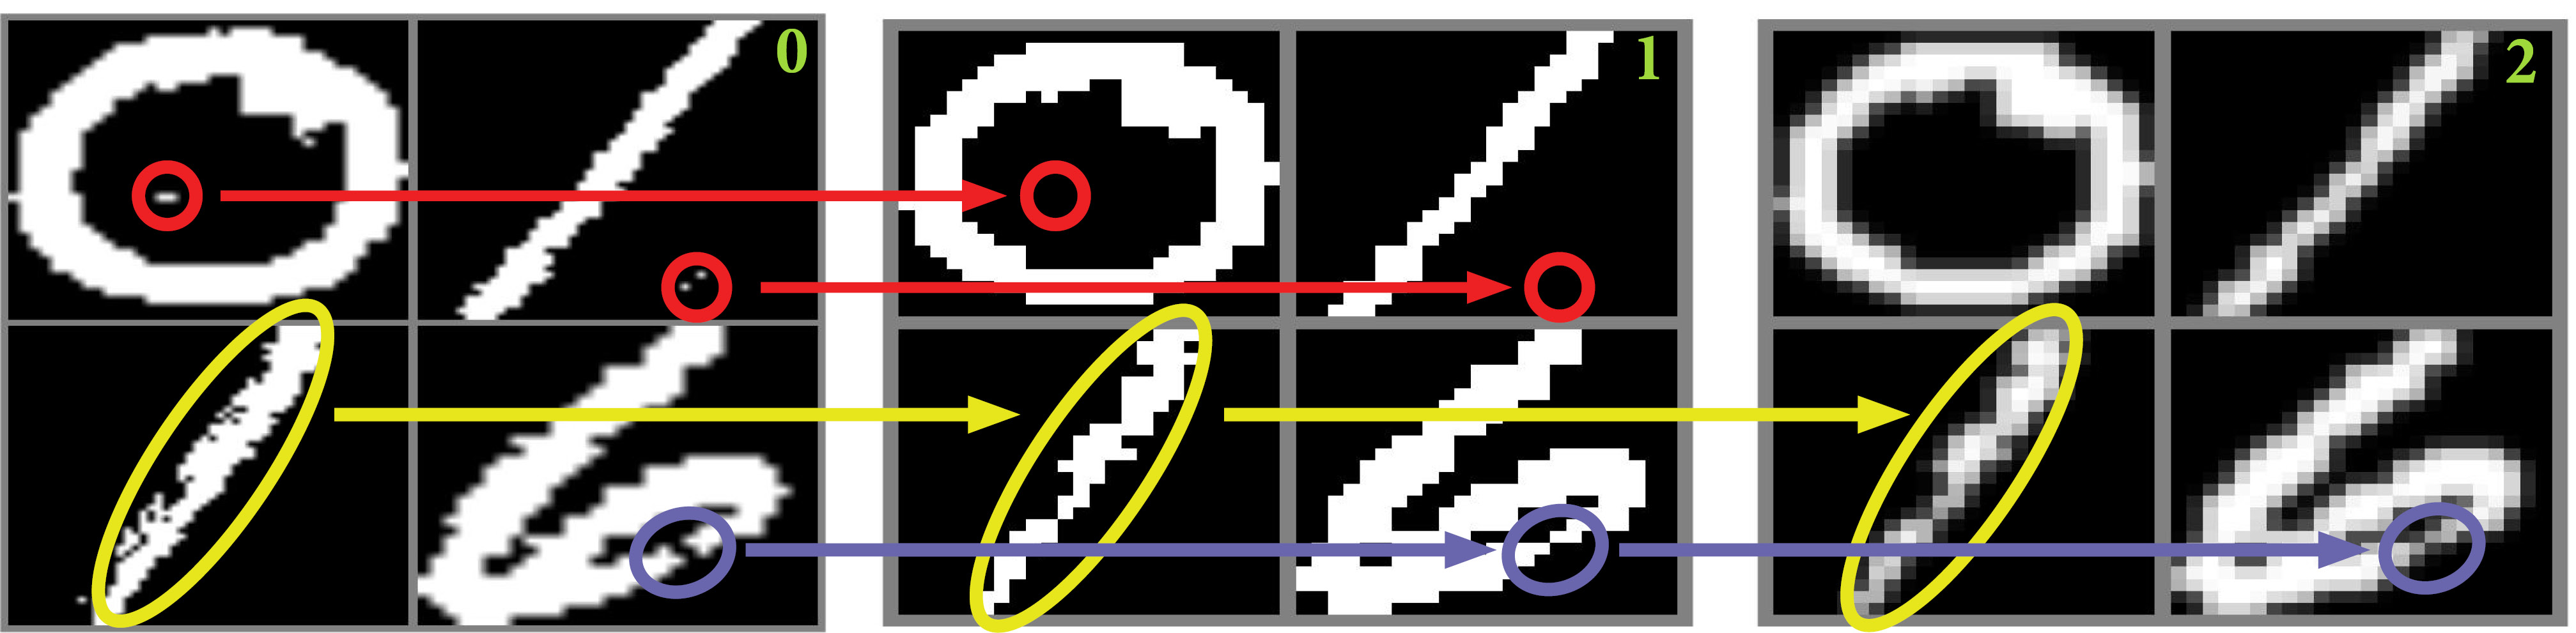
\includegraphics[scale=0.45]{images/Image_Prepros.jpg}
	\caption{Effect the pre-processing has on certain defects in the images. Step 1 removes single pixels and small blobs using \texttt{bwmorph.m} and \texttt{bwareaopen.m}. Step 2 adds a gaussian filter, to reconnect broken digits and smooth out any rough edges.}
	\label{fig:Image_Prepros}
\end{figure}
\newpage
\section{Classifier Design Process}
\label{sec:ClasDes}
As stated in the introduction, a classifier had to be build for two different cases. For both cases, a similar design approach was used. \begin{enumerate}
	\item Investigate amount of data and use the theory to choose an initial representation method
	\item Train simple classifiers based on the chosen representation method
	\item Perform evaluation
	\item If the performance does not meet the requirements, go back to the theory
	\item If the performance meets the requirements, optimise the system
\end{enumerate}
This approach is visualised in figure \ref{fig:case_design}.
\begin{figure}[H]
	\centering
	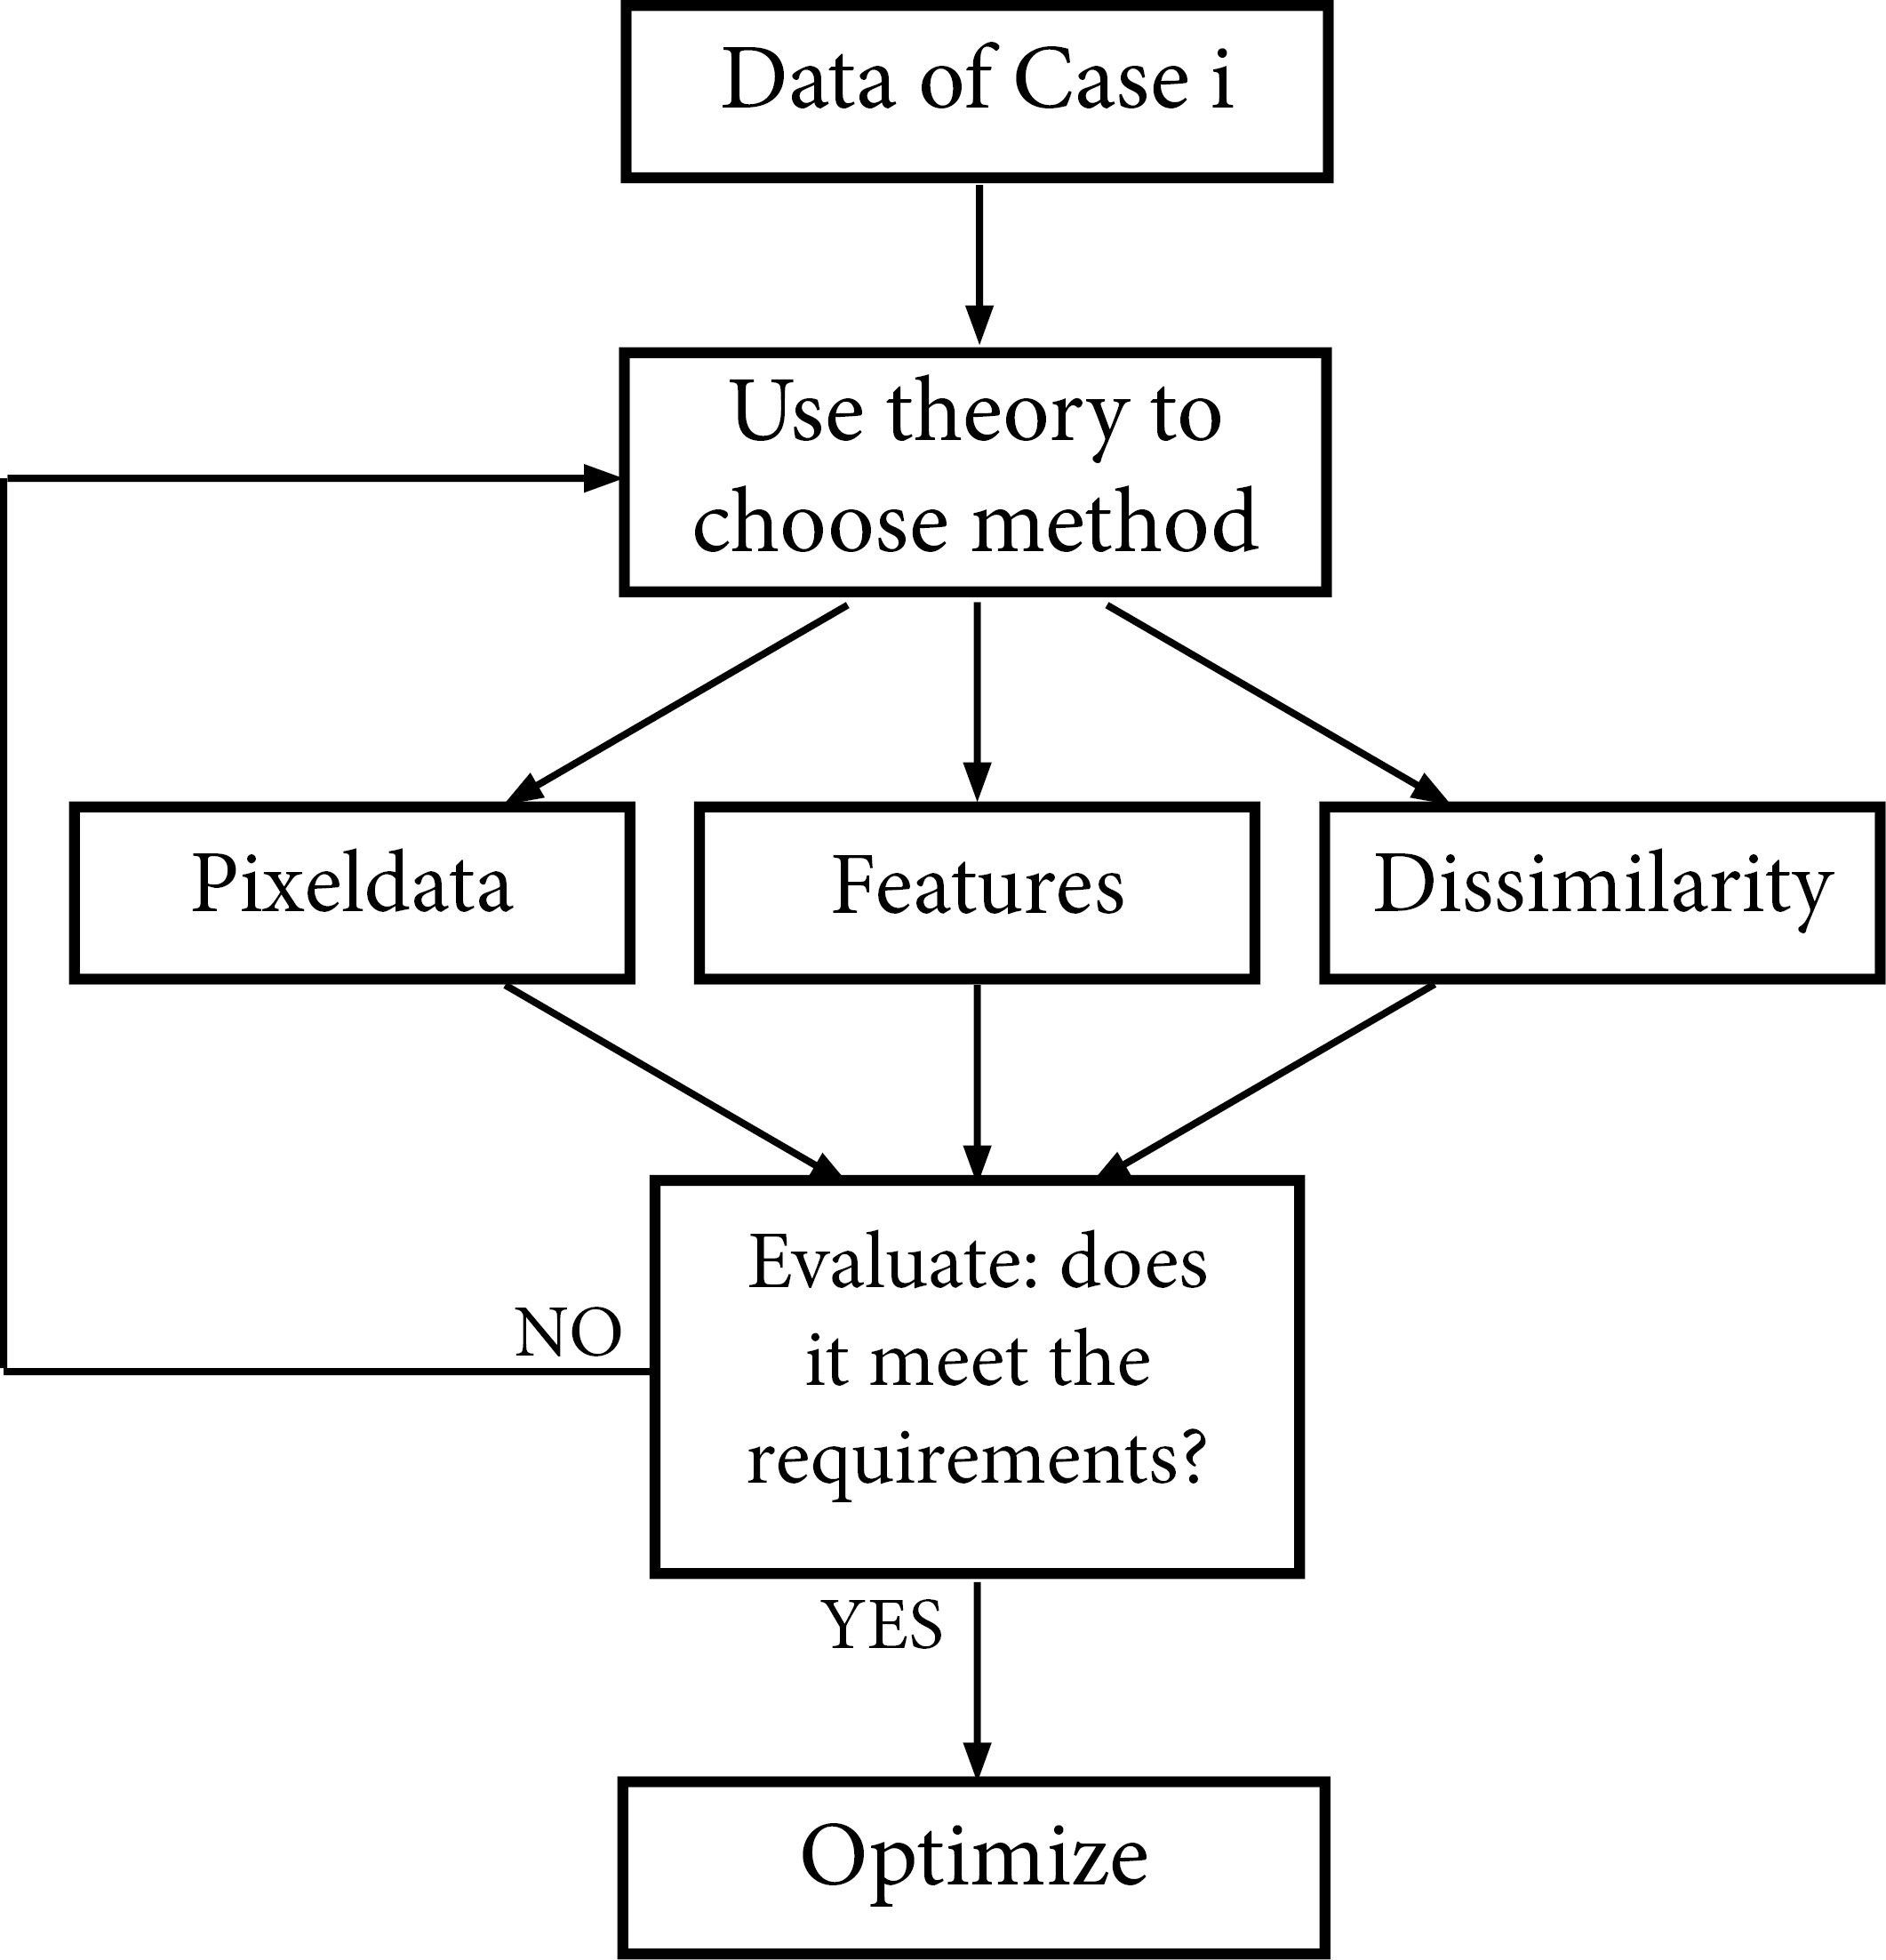
\includegraphics[scale=0.55]{images/Case_Design.jpg}
	\caption{Design-process to determine the best representation method for each of the two cases described in the Introduction.}
	\label{fig:case_design}
\end{figure}
\noindent The image processing described in chapter \ref{sec:ImPros} was kept the same for both cases, since it is a very subtle processing and will benefit all potential methods.

\newpage
\section{Case 1}
\label{sec:Case1}
\textbf{Case Summary:} Design a system for training on all cheques at once. The system must be able to correctly classify the handwritten digits after being trained on at least 200 objects per class.\\
\\
Per representation method, the best classification option will be investigated. All error rates of the different classifying algorithms were estimated using cross-validation using 10 folds.\\

\subsection{Representation by Pixels}
\subsubsection*{Density Estimating Classifiers}
In this scenario the classifying system is trained once, and then applied in the field. This means that all available data can be used as training input, which results in 1000 objects per class, and 10.000 objects in total. (1000 zeros, 1000 ones, etc.) Large datasets facilitate classification using non-parametric density estimating classifiers. Classifiers of this type are known to perform very well when large datasets are available. After the image preprocessing was carried out as explained above, several density estimating classifiers were tested: Parzen density estimating classifier, and k-nearest neighbors classifiers for k = 1,2,3. Although these classifiers are sensitive to uneven scaling of different features, rescaling of feature vectors is not necessary, because all pixel values are within the same range. The results can be seen in table \ref{tab:density}. The images used are 16x16 pixels, which results in a 256 dimensional feature-space. The Parzen classifier optimizes its ‘width’ parameter iteratively. The error rates for these classifiers pass the threshold of 5\% already. The error per digit class can be observed in figure \ref{fig:errorpdigit}. This shows that errors in ‘8’ and ‘9’ are high for all classifiers, as well as the error for ‘3’, ‘4’ and ‘5’ to a lesser extent. \\
For reference, a quadratic discriminant classifier (QDC) was added, which is parametric in contrast to the non-parametric classifiers mentioned above. The QDC performs significantly worse than the other classifiers, because it suffers more from the ‘curse of dimensionality’. That is to say that the performance of the classifier benefits from adding more features only up to a certain point, after which the error will rise with extra features added. The ‘curse of dimensionality’ implies that reducing the number of features might decrease the error attained by the classifiers.
\begin{table}[H]
	\centering
	\caption{Overview of the Density-Estimating classifiers and their estimated error.}
	\label{tab:density}
	\begin{tabular}{l|lllll}
		Classifier      & Parzen & 1-NN   & 2-NN   & 3-NN   & QDC    \\ \hline
		Estimated error & 0.0277 & 0.0280 & 0.0343 & 0.0321 & 0.2125
	\end{tabular}
\end{table}
\begin{figure}[H]
	\centering
	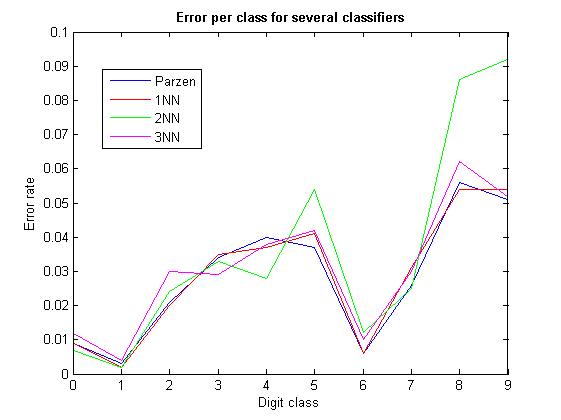
\includegraphics[scale=0.8]{images/pr_figure_2.png}
	\caption{Error per class for different non-parametric density-estimating classifiers.}
	\label{fig:errorpdigit}
\end{figure}
\subsubsection*{Feature Reduction}
Because of the large number of features in the original data set (16x16=256 pixel values) and large number of objects, any feature selection method, especially backwards propagating, will take a significant amount of time. For this reason feature selection methods were discarded, and feature extraction methods were investigated further. \\
The most frequently used feature extraction technique is Principal Component Analysis (PCA). In the PCA-algorithm, it is possible to indicate how much of the total variance should be preserved in the newly created features. The cross-validated error was calculated for the same classifiers as above after applying PCA using values of 0.90 to 0.95 of variance preservation. Results can be seen in table \ref{tab:PCA}. It is remarkable that the performance of the Parzen classifier deteriorates dramatically, while the performance of the 1-NN classifiers decreases only slightly, and the QD-classifier improves a lot, benefitting from the reduced dimensionality. Note that PCA is an unsupervised method, or in other words: it does not take the class labels or resulting performance of the classifiers into account when choosing new features. This explains the decreased performance of some of the classifiers after using PCA. \\
Pca is sensitive to the scaling of the features. Therefore it is recommended to normalize the variance of the features before applying PCA. In the case of pixel values, however, the data is inherently normalized, because all feature values are in the same range. Applying variance normalization will actually worsen the performance in this case, because it enhances the noise coming from pixels with very low variance. For example: the pixel in the top-left corner will practically always be black, so it has a very low variance. Rescaling will enhance the variance in this pixel, which has unwanted effects. \\
Addressing the poor performance of the parzen classifier after the application of PCA: even when using PCA to just decrease the dimensionality by 1, from 256 to 255 features, the performance decreases dramatically: from an error of approximately 3\% to an error of 13,57\%.  It is not clear why nearest neighbour algorithms do not seem to suffer from this problem. It might be that the parzen-algorithm suffers from an overlooked effect of PCA. Both the scaling of variance and moving the mean to the origin were empirically ruled out as possible solutions. \\
The (significantly improved) performance per class for the QD-classifier after applying PCA is compared to the performance as seen in figure \ref{fig:errorpdigit}, in figure \ref{fig:errorpdigit2}. It is noteworthy that the values of the QDC curves differ dramatically from the curves for the non-parametric classifiers without dimension reduction. For some classes QDC performs significantly better, while for others the ranking is inverted. This fact can be exploited using classifier combining.
\begin{table}[H]
	\centering
	\caption{Overview of the performance of the classifiers after applying PCA, with different values for the preserved variance.}
	\label{tab:PCA}
	\begin{tabular}{l|llllll}
		Preserved variance       & 0.90   & 0.91   & 0.92   & 0.93   & 0.94   & 0.95   \\
		Resulting dimensionality & 41     & 44     & 48     & 53     & 58     & 65     \\ \hline
		Parzen                   & 0.1122 & 0.1125 & 0.1134 & 0.1136 & 0.1159 & 0.1176 \\
		1-NN                     & 0.0304 & 0.0305 & 0.0314 & 0.0292 & 0.0297 & 0.0297 \\
		QDC                      & 0.0354 & 0.0354 & 0.0375 & 0.0379 & 0.0383 & 0.0361
	\end{tabular}
\end{table}
\begin{figure}[H]
	\centering
	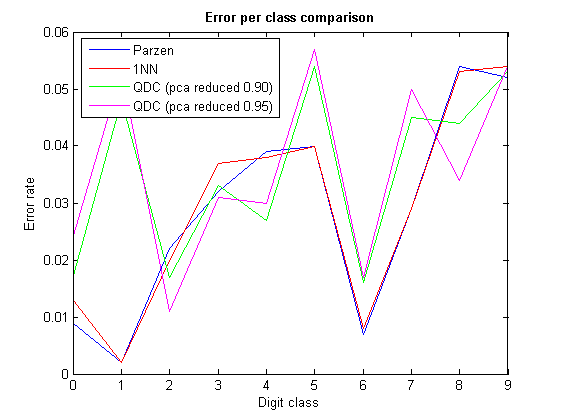
\includegraphics[scale=0.8]{images/pr_figure_3.png}
	\caption{Comparison of the error per class for different classifiers.}
	\label{fig:errorpdigit2}
\end{figure}
\subsubsection*{Combining}
Since the different classifiers in figure \ref{fig:errorpdigit2} perform well for different digit classes, the one alternately performing better than the other, it might be beneficial to combine them. Combining can be carried out using different combining rules. The following combining rules will be investigated: product rule, max rule, mean rule, median rule, min rule. Parzen is to be combined with PCA + QDC, for two different values of variance preservation, as is 1-NN. The result can be seen in table \ref{tab:comb}. The combination using the product rule of Parzen and QDC (after application of PCA preserving 90\% of the variance) offers the best result. The error rate per class can be seen in figure \ref{fig:errorpdigit3}. Except for the digits ‘0’ and ‘1’ (for which Parzen performs best), the combination performs better than the two original classifiers. The ‘9’ is still the digit with the highest classification error.
\begin{table}[H]
	\centering
	\caption{Estimated error for different combinations of classifiers, using different combination rules.}
	\label{tab:comb}
	\begin{tabular}{l|lllll}
		Combining rule                                             & Product & Max    & Mean   & Median & Min    \\ \hline
		\begin{tabular}[c]{@{}l@{}}Parzen\\   + QDC90\end{tabular} & 0.0222  & 0.0271 & 0.0263 & 0.0276 & 0.0333 \\
		\begin{tabular}[c]{@{}l@{}}Parzen\\   + QDC95\end{tabular} & 0.0225  & 0.0274 & 0.0276 & 0.0267 & 0.0367 \\
		\begin{tabular}[c]{@{}l@{}}1-NN\\   + QDC90\end{tabular}   & 0.0361  & 0.0281 & 0.0282 & 0.0285 & 0.0354 \\
		\begin{tabular}[c]{@{}l@{}}1-NN\\   + QDC95\end{tabular}   & 0.0382  & 0.0298 & 0.0281 & 0.0281 & 0.0369
	\end{tabular}
\end{table}
\begin{figure}[H]
	\centering
	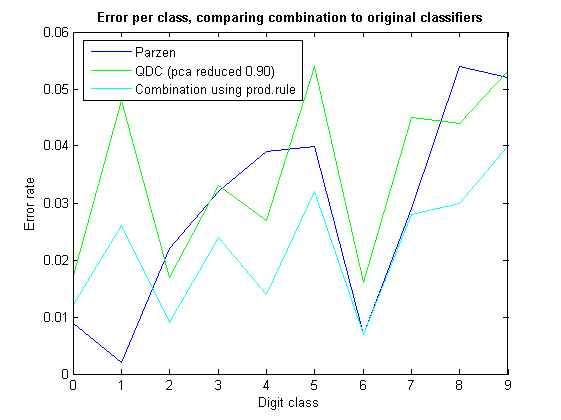
\includegraphics[scale=0.8]{images/pr_figure_4.png}
	\caption{Overview of the error per class of the two original classifiers and their optimal combination.}
	\label{fig:errorpdigit3}
\end{figure}
\subsubsection*{Support Vector Machines}
Support Vector Machines (SVM) are known to be especially useful for classifying in high dimensional feature spaces, which is a major advantage when analyzing pixel data. However, the lengthy runtime of the SVM-algorithm is a major disadvantage. Because of the limited time available to analyze the different classifiers, the SVM-algorithm was discarded as a viable option. Once the SVM is created, the runtime of using it to classify and to test it is relatively short. But tweaking and testing it over and over would have taken a significant amount of time. Furthermore, enough training data is available to make adequate density estimations.

\subsubsection*{Preliminary Conclusion} for Case 1 with a representation by pixels, the combining classifier (product rule) of Parzen and QDC (after PCA reduced 0.9) gives the best performance, with an error of 0.0222.

\subsection{Representation by Features}
At first glance, the feature representation approach is not the most suitable for scenario 1. Given a large dataset, the performance of the classifiers will benefit from a relatively large number of features. The image analysis methods included in the PRToolbox give 14 features we deemed useful (see Case 2 for a more in-depth discussion of this choice). A number which is predicted to be insufficiently high for achieving an error rate comparable to the rates accomplished using the pixel data approach. Furthermore, because the blob-removal discussed in \ref{sec:ImPros} was not implemented for the large dataset (due to a too large computation time), this method might perform sub-optimal.\\
In order to verify this prediction some indicative tests were carried out, using various classifiers on the dataset containing the extracted features. The tested classifiers are: nearest mean classifier (nmc), Parzen density estimating classifier, 1-nearest neighbor classifier, linear discriminant classifier (ldc), logistic classifier (loglc), and quadratic discriminant classifier. In table \ref{tab:feat} the results of these test are shown. For the relevant classifiers (NMC, Parzen, 1-NN) the features were normalized before attempting classification. The resulting error rates are significantly higher than the errors attained above, and have no prospect of improving by feature reduction, because the original dimensionality is low.
\begin{table}[H]
	\centering
	\caption{Overview of the estimated error for different classifiers based on a feature-representation.}
	\label{tab:feat}
	\begin{tabular}{l|llllll}
		Classifier                                                  & NMC    & Parzen & 1-NN   & LDC    & LOGLC  & QDC    \\ \hline
		\begin{tabular}[c]{@{}l@{}}Estimated\\   error\end{tabular} & 0.4454 & 0.3472 & 0.2032 & 0.2178 & 0.1863 & 0.3207
	\end{tabular}
\end{table}
\subsubsection*{Preliminary Conclusion}
The hypothesis is accepted as true, and the feature representation approach is discarded for the large dataset case. The best performing classifier is a Logistic Classifier, with an error of 0.1863. This is not sufficient to surpass the pixel-representation. The feature-representation approach will be dealt with in some more depth in scenario 2, later in this report.

\subsection{Representation by Dissimilarities}
While the main focus for scenario 1 was on the pixel data representation, a brief look was had at a dissimilarity-representation for the NIST-digits. The dissimilarity-representation offers a better outlook than the feature-representation, because it allows for higher dimensionalities. In the dissimilarities approach ‘distances’ to certain ‘prototype’ digits are used as a means for classification. Both the choice of distance measure and the choice of prototype influence the error rate of the resulting classifier. To be able to quickly test the effectiveness of the dissimilarity representation, only the Euclidian distance measure was used on case 1. Results are averaged over 3 randomly sampled sets of 10 prototypes per class. The samples remaining in the dataset were used for training (990 samples per class). The results of this quick experiment can be seen in table \ref{tab:diss}. The tested classifiers match those tested for the feature representation.
\begin{table}[H]
	\centering
	\caption{Overview of the estimated error for different classifiers based on a dissimilarity-representation.}
	\label{tab:diss}
	\begin{tabular}{l|llllll}
		Classifier                                                  & NMC    & Parzen & 1-NN   & LDC    & LOGLC  & QDC    \\ \hline
		\begin{tabular}[c]{@{}l@{}}Estimated\\   error\end{tabular} & 0.3487 & 0.0567 & 0.0638 & 0.0741 & 0.0510 & 0.0452
	\end{tabular}
\end{table}
\subsubsection*{Preliminary Conclusion}
The results have improved compared to the feature representation approach, but not exceeded the results of the pixel data approach. PCA was applied to reduce the dimensionality, but this had an adverse effect in this case. The best performing classifier for this representation was a QDC with PCA, with an estimated error of 0.0452. \\
To improve results, representative prototypes (a set of very averagely written digits) could be chosen, instead of picked randomly, and alternative dissimilarity measures could be investigated (see Discussion).\\
\subsection{Final Conclusion and Evaluation for Case 1}
As can be seen in table \ref{tab:concase1}, the combination of a Parzen classifier and a QD-classifier applied after PCA, combined using the product rule, yields the best result for scenario 1. 
\begin{table}[H]
	\centering
	\caption{Overview of the best performing classifiers per representation, and their errors.}
	\label{tab:concase1}
	\begin{tabular}{l|ll}
		Representation  & Best Classifier               & Estimated Error \\ \hline
		Pixeldata       & Combination of Parzen and QDC & 0.0222          \\
		Features        & Logistic                      & 0.1863          \\
		Dissimilarities & QDC                           & 0.0452         
	\end{tabular}
\end{table}
\noindent The error of the chosen combined classifier was determined more accurately using cross-validation employing 10 folds, and 10 repetitions. This way some measure of stability can be given, using the standard deviation between the repetitions. The cross-validation yields an error rate of 0.0219 with standard deviation 5.3125e-4. The standard deviation is very small, which means the classifier is stable for different test sets (picked at random from the original dataset).\\
The benchmark test (using \texttt{NIST\_eval.m}) yields an error rate of 0.0260 for the chosen classifier for scenario 1. This error is below the desired threshold of 5\%, but is slightly higher than the error found using cross-validation. This might be a result of different class frequencies in the evaluation set compared to the training dataset. In the test set all classes were represented equally often, but in the evaluation set a more realistic class distribution could have been used, increasing the total error rate if this digit has a larger than average misclassification rate. It would not be strange if the frequency of ‘9’ (which has the highest error rate for the used classifier) occurring on bank cheques was slightly higher in practice, due to prices of products often looking like -.99. Note that this last remark is speculation, as there is no way to verify the contents of the evaluation set.





\newpage
\section{Case 2}
\label{sec:Case2}
\textbf{Case Summary:} Design a system for training on each batch of cheques to be processed. The system must be able to correctly classify the handwritten digits after being trained on a maximum of 10 objects per class.\\
\\
\noindent The amount of data available in this case poses some restrictions. While a pixel-data representation worked very well in Case 1, it is likely to have too little data to work with in this case. Some more prior knowledge is needed to handle these batches of cheques. One way of doing this is by letting the system recognize certain distinct properties of the digits. A straight-forward way of doing this is by using a feature representation of the objects. A more abstract way is using a dissimilarity representation.
\\
\subsection{Representation by Features}
To start out, features were chosen as the best representation for this case. The function \texttt{im\_features} from the prtools-toolbox was used to compute 14 different features of all the images in the pre-processed database. Because the amount of features is relatively high compared to the amount of data that is used, some form of feature reduction needs to by applied. MatLab's forward feature selection (\texttt{featself}) was used initially to get a sense for the features that should be used and the features that could be omitted. This was done for four cases; with and without scaling of the data, and with and without implementing a separate test-set in the \texttt{featself} function. The resulting performance can be seen in figure \ref{fig:featsel_perf}
\begin{figure}[H]
	\centering
	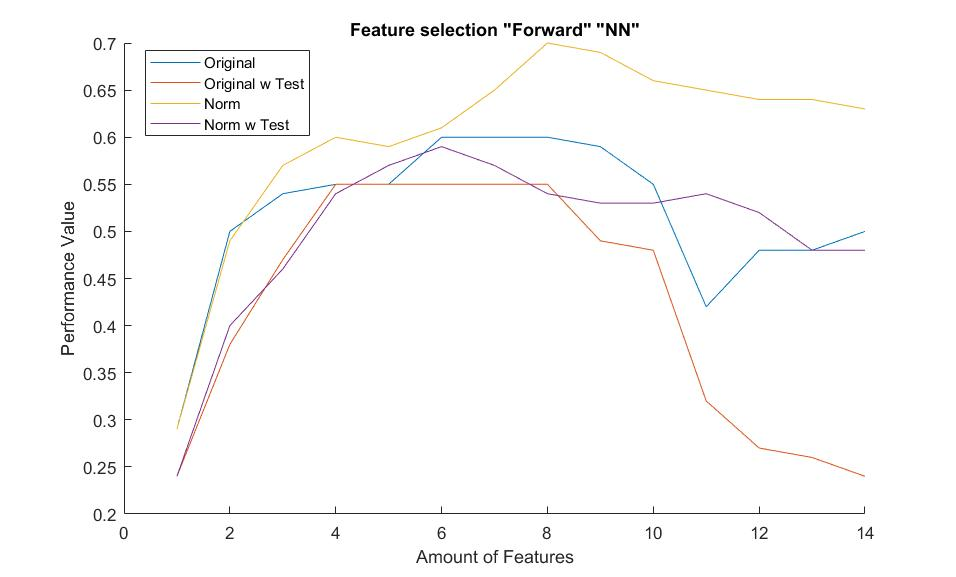
\includegraphics[scale=0.45]{images/featsel_perf.jpg}
	\caption{Performance of features selected by forward feature selection. Both scaling and non-scaling, and with or without test-set are shown.}
	\label{fig:featsel_perf}
\end{figure}
\noindent As can be seen in the figure, there are a lot of differences between the different parameters. There appears to be an optimal amount of features however, somewhere between 4 and 12. In order to get a better grip on which features to use, different feature selection strategies were compared. After the forward selection, the backward and the plus-2-takeaway-1 were tested. This is was done for both the '1-Nearest Neighbor' and the 'Summed Mahalanobis distances' criterion. All these methods indicated that there was an optimum somewhere between 4 and 12 features. However there seemed to be no correlation between which of the features belonged to this optimal set. Therefore a brute force approach was taken. Each possible combination between 3 and 14 features was used for an error-calculation (using the \texttt{testc}  function of PRTools) of four different classifiers (Fischer's Classifier, Linear Classifier, Nearest Mean Classifier and a Nearest Mean Classifier trained on normalized data). After running this setup overnight, the following results were obtained: (see figure \ref{fig:feat_bf_error}).
\begin{figure}[H]
	\centering
	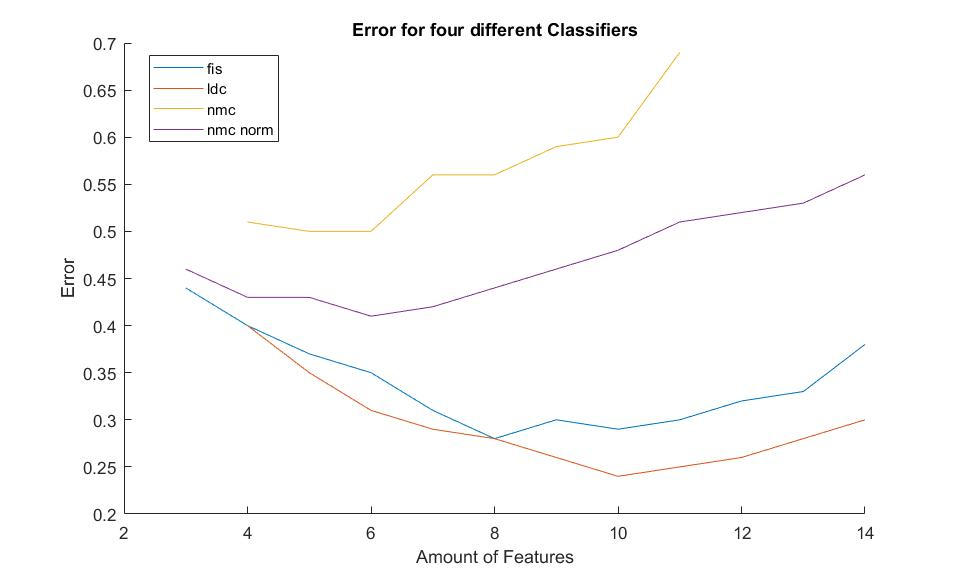
\includegraphics[scale=0.45]{images/feat_bf_error.jpg}
	\caption{Error of different combinations of features for four different trained classifiers; Fischer's (\texttt{fischerc}), Linear Bayes-Normal (\texttt{ldc}), Nearest Mean (\texttt{nmc}) and a normalised version of Nearest Mean.}
	\label{fig:feat_bf_error}
\end{figure}
\noindent This figure shows the lowest error obtained with a certain amount of features. It suggests the optimal amount is 10. It also shows that the Linear Classifier will probably perform best, although even its best error is not under the 25 percent yet. \\
Next, for the LDC classifier only, these 10 features were tested on different datasets. The result of this was a big fluctuation in errors between datasets, which implies that the set of 10 features were only optimal for one particular dataset. Therefore another brute force approach was used to test all possible combinations of 9 to 12 features on different datasets. In figure \ref{fig:feat_jumps} the error of every combination of 9 features can be seen. Very noticeable are the large drops and jumps in the graph, visualised with the orange line below it. After close inspection of the used features at these points, it was discovered that every increase in error corresponded to the same four features being added, namely 'Convex Area', 'Conves Hull', 'Convex Image' and 'Eccentricity'. A similar pattern was recognized in the other results. It was decided to omit these features, leaving the final dataset with the desired amount of 10 features.
\begin{figure}[H]
	\centering
	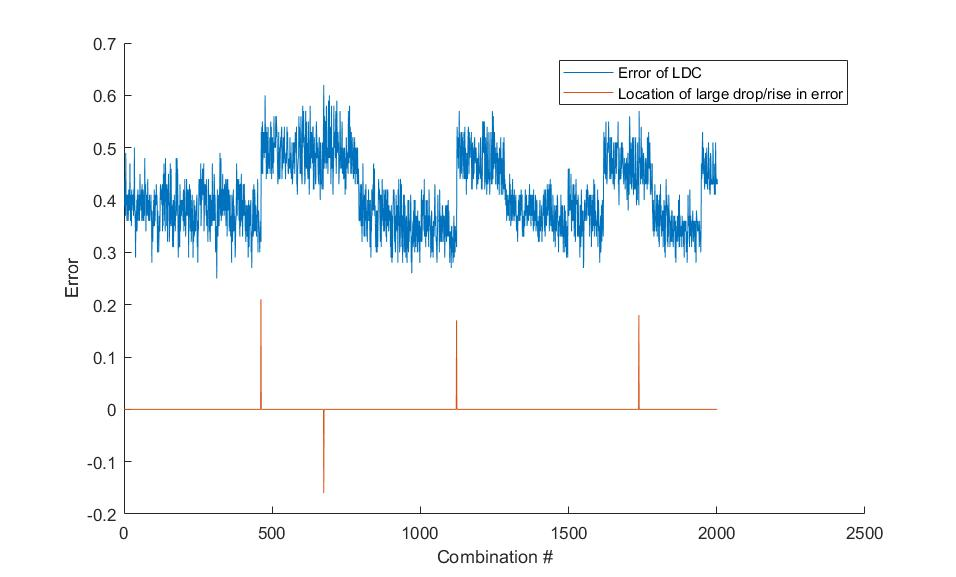
\includegraphics[scale=0.45]{images/feat_jumps.jpg}
	\caption{Error of the LDC-classifier for each possible combination of 10 out of 14 features. The orange line indicates places with a large increase or decrease in error-value.}
	\label{fig:feat_jumps}
\end{figure}

\subsubsection*{Preliminary Conclusion}
\noindent At this time, the complete system consisted of a Linear Classifier (LDC) trained on the dataset from which 10 out of 14 features were selected. Sadly though, testruns of the algorithm yielded an error of 30\%, as can be seen in figure \ref{fig:feat_jumps}. Since this is too low to meet the requirements, a different approach was taken. \\

\subsection{Representation by Dissimilarity}
It was decided that more information needed to be intrinsic in the system in order for it to be able to correctly classify the digits with the small trainingset Case 2 provides. Going back to the theory, dissimilarity-representation seemed to be able to do this. By picking a few representative examples of each digit by hand (the prototypes) and calculating the distance of the remaining objects to these prototypes, correct classification should be possible. \\
\noindent To get a first test of this principle, it was tried to first filter out all the zeros. 90 samples per class were taken, three representative zeros were choosen, and the distance between all objects and these three zeros was calculated using MatLab's \texttt{proxm.m} function. In figure \todo{INSERT FIGURE waar die zeros goed geseparate zijn! misschien ff met maar 10 per class, zoals deze case voorschrijft.} a clear grouping of all the zeros can be observed, and this group can be separated from the rest of the objects easily. This was done for various distance measures. City-blok distance seemed to give the best result. \todo{tabelletje met andere distance measures waaruit blijkt dat dit inderdaad zo is? er schijnt ook een paper te zijn, even naar verwijzen. VERWIJZEN NAAR PAPER, en zeggen dat het in image goed werkt} \\
\noindent The next step is to try this with every digit. Ten samples per class were taken, and in stead of selecting the prototypes manually, all objects were given as prototypes. This meant a dataset of 100 samples, each of them having 100 features. With this, an error of below 25 percent was reached. \todo{ldc word getrained. QDC ook. vergelijking: QDC was beduidend slechter.} \\
\noindent The created dataset is very large however, so feature reduction might be in place. 
featsellr en PCA geprobeerd. wordt slechter. qdc nog slechter. 

\subsubsection*{Preliminary Conclusion}
bla

\subsection{Representation by Pixels}
bla

\subsubsection*{Preliminary Conclusion}
bla

\subsection{Final Conclusion and Evaluation for Case 2}
\begin{table}[H]
	\centering
	\caption{Overview of the best performing classifiers per representation, and their errors.}
	\label{tab:concase1}
	\begin{tabular}{l|ll}
		Representation  & Best Classifier               & Estimated Error \\ \hline
		Pixeldata       &  & 0.0222          \\
		Features        & LDC with 10 out of 14 selected features                      & 0.30          \\
		Dissimilarities &                            &          
	\end{tabular}
\end{table}
\newpage
%\section{Classifier Evaluation}
\label{sec:Eval}

\subsection{Evaluation of Image Processing}

\subsection{Evaluation of Case 1}

\subsection{Evaluation of Case 2} 
%\newpage
\section{Discussion and Conclusion}
\label{sec:DiscConcl}

Include a section Recommendations to your report, in which you advise your client in detail on possible steps to improve performance in light of the overall system they are constructing. \\
For example:\\
will having more training data help?\\
would other features help? \\
does the application require reject options? \\
does a single classifier suffice for all digits on a bank cheque? \\
what is the role of time constraints?

  




\end{document}